\documentclass[a4paper,doc,natbib]{apa6}
\usepackage[english]{babel}
\usepackage[utf8x]{inputenc}
\usepackage{amsmath}
\usepackage{graphicx}
\usepackage{caption}
\usepackage{subcaption}
\title{Research proposal: The anchoring effect in calorie estimation}
\shorttitle{The anchoring effect in calorie estimation}
\author{Yasin G\"{u}l \and Arjan Broer}
\affiliation{Open University of the Netherlands}

\abstract{Obesity is a world-wide problem, caused in part, by the easy access to high caloric foods. We here propose a study to investigate whether the anchoring effect can influence people into overestimating the number of calories in foods, which may aid in choosing lower caloric foods or to consume less. In the study, participants will be presented with foods and will be asked to estimate the number of calories in those foods. Before being asked the calorie contents, participants will sometimes be presented with an anchoring question, which asks them to estimate whether the food has less or more calories than a specific anchoring value. The hypothesis that subsequent calorie estimates will be biased towards the anchoring value, will be tested by comparing low and high anchoring values with situations in which no anchoring value is provided.}
\begin{document}

\maketitle

\section{Background}

Obesity is a significant problem in many parts of the world. For example, in Europe, the prevalence of obesity (a body mass index of over 30) was found to range from 4.0\% to 28.3\% in men and between 6.2\% and 36.5\% in women \citep{berghofer2008obesity}. In the US obesity prevalence is even higher with an estimated 39.8\% of adults being obese between 2015 and 2016 \citep{hales2017prevalence}. 

Obesity increases the risk of various health conditions, such as hypertension and kidney disfunction \citep{hall2019obesity}, diabetes \citep{schnurr2020obesity} and gallbladder disease \citep{zahra2019link}. Recently obesity has also been implicated in a worse outcome of a Covid-19 infection \citep{hussain2020obesity}. Tackling obesity is therefore important to tackle ill health in general.

People are inherently poor at estimating the caloric contents of foods. People have been found to underestimate the caloric contents of foods that are considered to be healthy \citep{chandon2007biasing} or labelled as `low fat' \citep{ebneter2013less}. Adding extra healthy ingredients to a dish can lead to lower estimates of calorie contents \citep{zhu2019extra}, while larger images can lead to higher estimates \citep{tal2021visual}. When foods are eaten together, people show difficulties keeping track of caloric contents when ordering multiple food items \citep{gustafson2019cognitive}, and it matters whether foods are served separate or mixed \citep{ai2021serving}. Likewise, menus with fewer items lead to higher calorie estimates of the foods that are on the menu \citep{kim2022impact}.

Given these context effects, it may be possible to directly influence people's estimates of calorie contents of foods. One such direct influence may be obtained by the anchoring effect \citep{furnham2011literature,tversky1974judgment}. The anchoring effect refers to the observation that when participants are first asked whether a value is lower or higher than an anchor value (e.g., `is the Eiffel tower smaller or larger than 100m?'), they are subsequently influenced by the anchor value when estimating the actual value (e.g., `how tall is the Eiffel tower?').

The anchoring effect has been observed across many domains, including general knowledge questions \citep[e.g.,][]{blankenship2008elaboration,epley2001putting},  estimating probabilities \citep{plous1989thinking}, legal judgements \citep{enough2001sentencing}, purchasing decisions \citep{ariely2003coherent}, and loan repayments \citep{stewart2009cost}. The anchoring effect occurs even if participants know that the anchors have been selected at random \citep{englich2006playing,tversky1974judgment}, and can be found with implausible anchor values \citep{strack1997explaining}. The anchoring effect is stronger when participants are in a low mood \citep{englich2009moody}, but weaker in participants with expertise in the domain \citep{wilson1996new,englich2009moody}, in participants with certain personality traits \citep{eroglu2010biases}, and participants with high self-confidence in their estimates \citep{wu2012role}. On the basis of these findings, various theories have been forward to explain the anchoring effect, including it being a heuristic mechanism \citep{tversky1974judgment} and the idea of `confirmatory search' \citep{chapman1999anchoring}.

\section{Research questions}

Given the consistent finding of the anchoring effect \citep{furnham2011literature}, and the poor ability of people to estimate the calorie contents of foods \citep[e.g.,][]{ebneter2013less}, it is highly plausible that the anchoring effect can also be observed when estimating calorie contents. The study will therefore address the following research questions:

\begin{description}
\item[RQ1.] Does the anchoring effect occur for calorie estimation in foods?
\item[RQ2.] Does this anchoring effect depend on the type of food?
\item[RQ3.] Do people who are confident in their calorie estimates have a smaller anchoring effect?
\item[RQ4.] Do people who check food labels have a smaller anchoring effect?
\end{description}


\section{Research methods}

\subsection{Participants}

Participants will be recruited during teaching sessions of the course `Interactive visualisation' at Tilburg University. Around 70 students take part in the course per year, and it is therefore expected that across two runs around 100 participants may be recruited for the study (not everyone may be able to attend the sessions or might want to take part).

\citet{shanks2020incidental} report pooled values for Cohen's $d$ for an anchoring study, finding values ranging from 0.19 to 0.41. With the 0.19 value, the expected sample will be too low (for a power of 0.8, computed with the `pwr' package in R, a per group sample of 435 will be needed). For a value of 0.41, the per group sample required to achieve a power of 0.8 is 94, which is still higher than the expected sample size. The study may therefore be underpowered.

The experiment will be run as part of a course, meaning that no approval will be required from the local ethics committee, provided that data cannot be traced back to individual participants, participants are not expected to be harmed by taking part, participants take part voluntarily, and the data are only used for teaching purposes.

\subsection{Apparatus}

The experiment will be conducted on participants' own laptops or computers available in the teaching areas. Presentation of the images and questions and collection of the responses will be controlled with the Opensesame environment \citep{mathot2012opensesame}. Images will be shown on the screen of the laptop and desktop computers, and responses will be collected with the mouse and the keyboard of these devices.

\subsection{Stimuli}

To reduce the testing time, increasing the chance that participants will complete the study, nine food items will be used, distributed across the three anchoring conditions (low, high and no anchor). Figure~\ref{fig:foods} shows the images of the nine foods that are used, while Table~\ref{tab:descriptions} provides the descriptions. Information about the calorie contents are obtained from website X. The anchors will be set by either dividing the actual calorie contents by 1.4 (low anchors) or by multiplying the actual calorie contents by 1.4 (high anchors).

\begin{figure}[h!]
\begin{subfigure}[b]{0.32\textwidth}
 \caption{Banana}
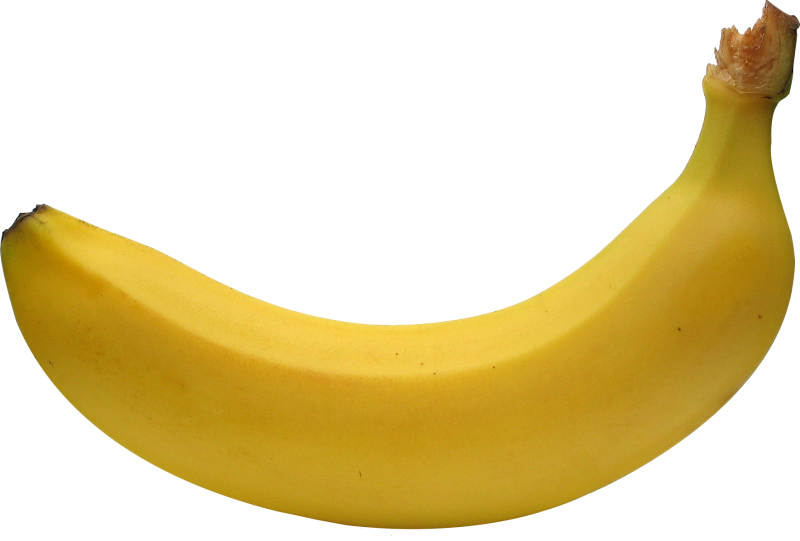
\includegraphics[width=0.95\linewidth]{Images/banana.png}
 \end{subfigure}
 \begin{subfigure}[b]{0.32\textwidth}
 \caption{Cake}
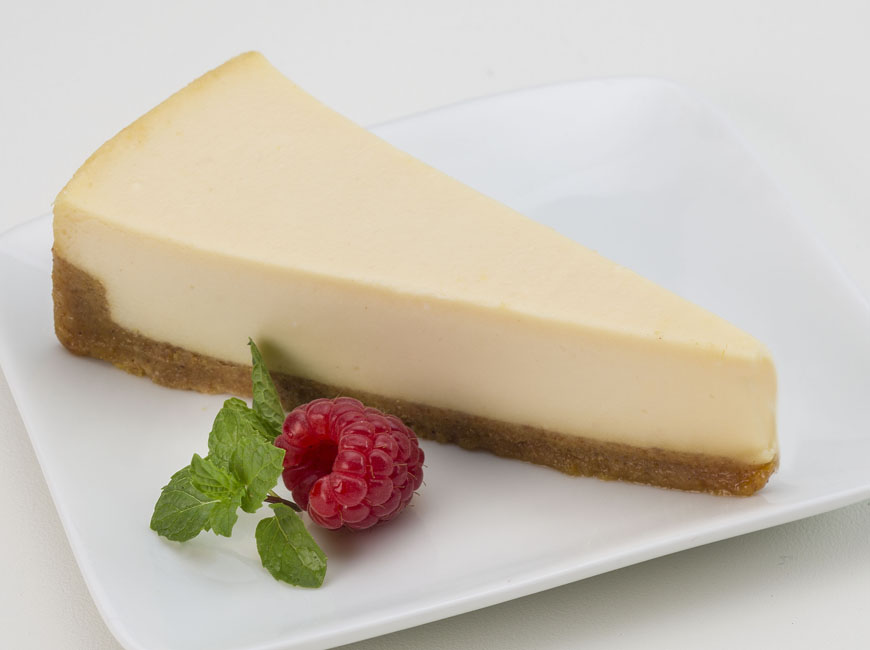
\includegraphics[width=0.95\linewidth]{Images/cake.jpg}
 \end{subfigure}
 \begin{subfigure}[b]{0.32\textwidth}
 \caption{Cheese}
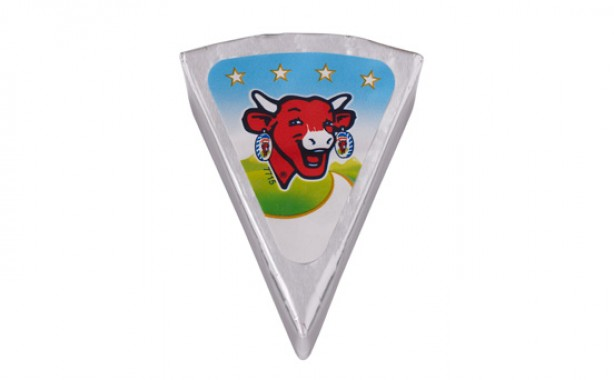
\includegraphics[width=0.95\linewidth]{Images/cheese.jpg}
 \end{subfigure}
\begin{subfigure}[b]{0.32\textwidth}
 \caption{Fries}
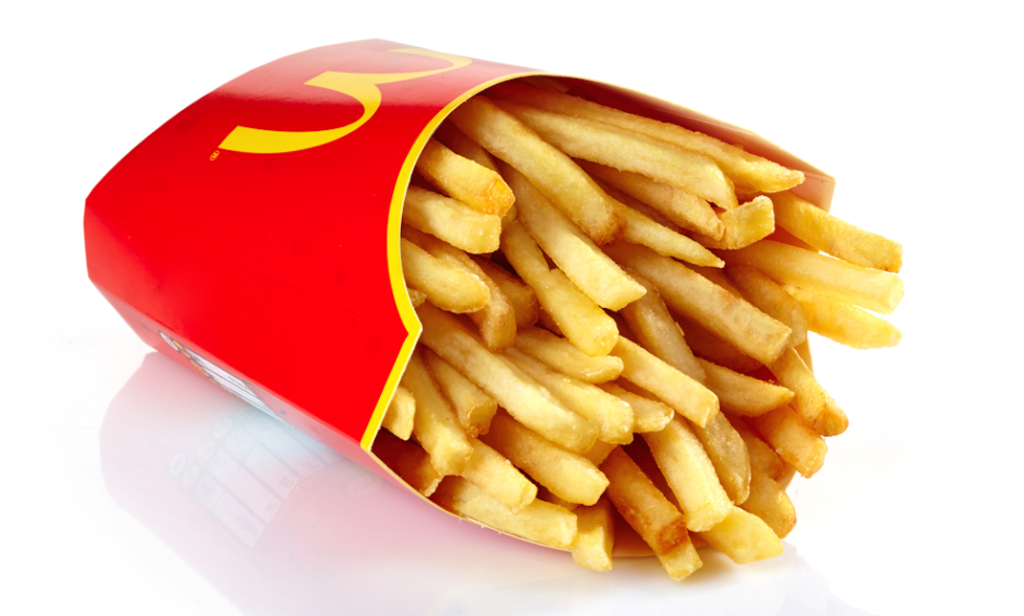
\includegraphics[width=0.95\linewidth]{Images/fries.png}
 \end{subfigure} 
 \begin{subfigure}[b]{0.32\textwidth}
 \caption{Honey}
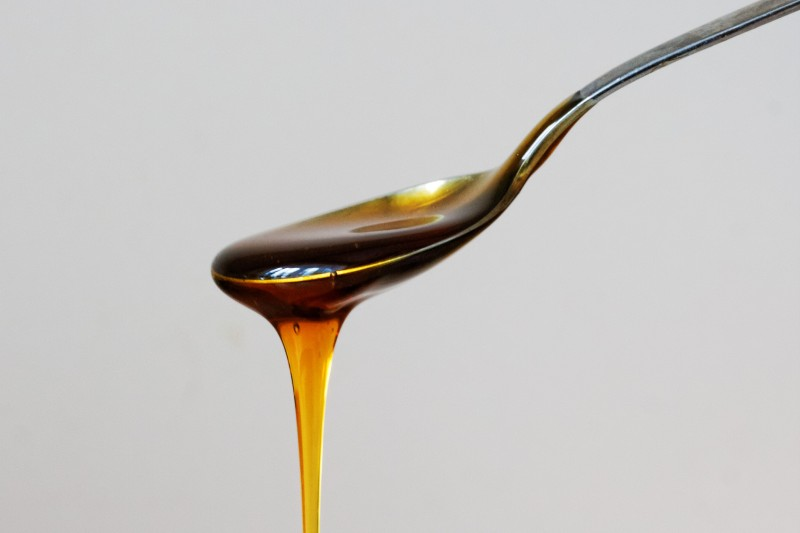
\includegraphics[width=0.95\linewidth]{Images/honey.jpg}
 \end{subfigure} 
  \begin{subfigure}[b]{0.32\textwidth}
 \caption{Mars}
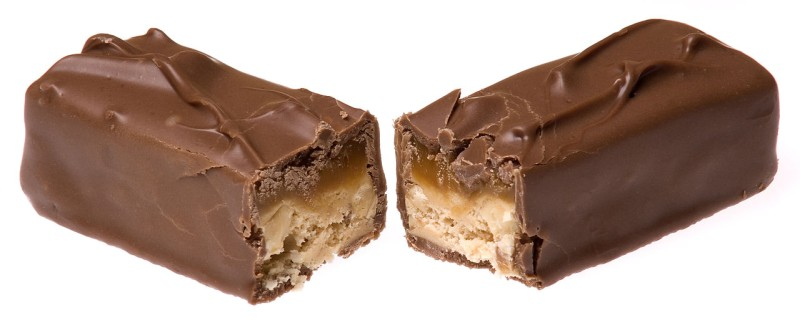
\includegraphics[width=0.95\linewidth]{Images/mars.jpg}
 \end{subfigure} 
   \begin{subfigure}[b]{0.32\textwidth}
 \caption{Peanuts}
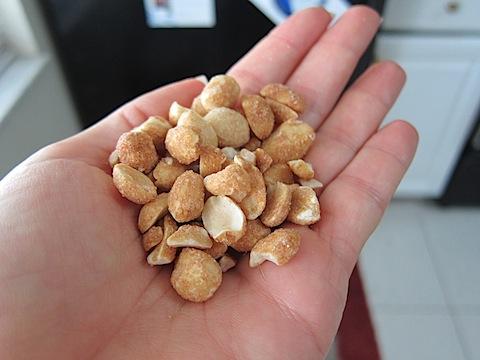
\includegraphics[width=0.95\linewidth]{Images/peanuts.jpg}
 \end{subfigure}
\begin{subfigure}[b]{0.32\textwidth}
 \caption{Pizza}
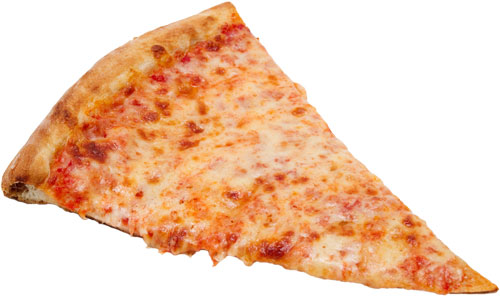
\includegraphics[width=0.95\linewidth]{Images/pizza.jpg}
 \end{subfigure}
 \begin{subfigure}[b]{0.28\textwidth}
 \caption{Wine}
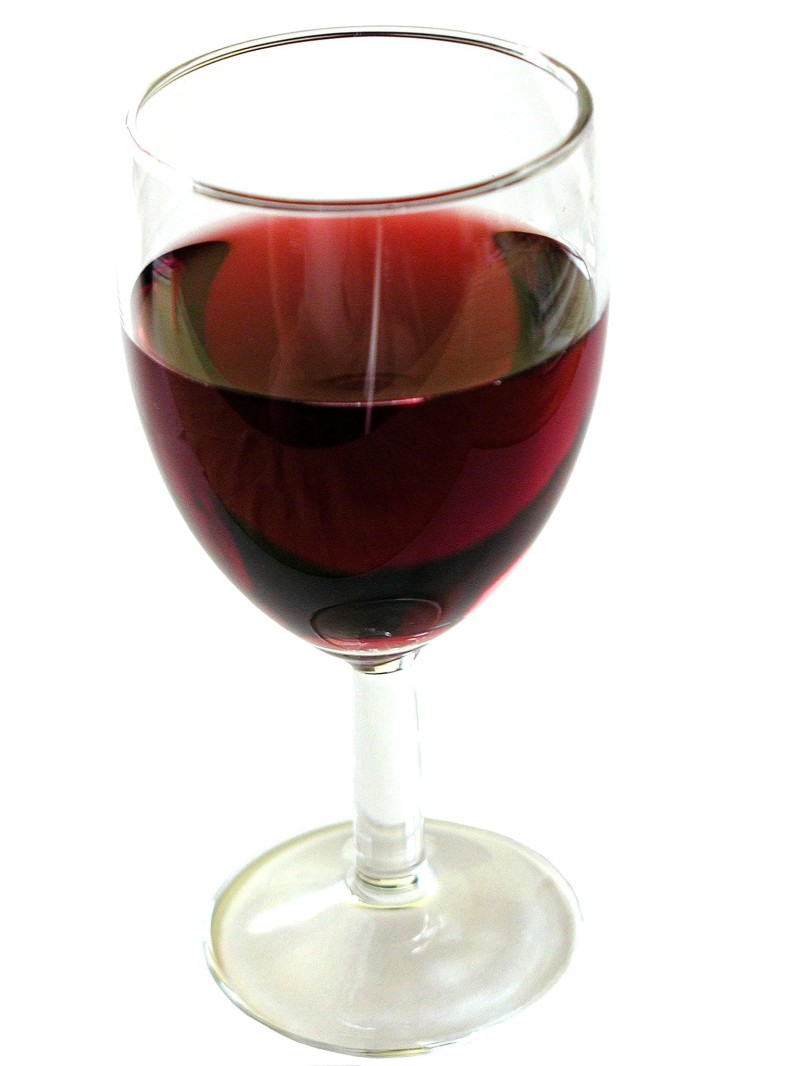
\includegraphics[width=0.95\linewidth]{Images/wine.jpg}
 \end{subfigure}
\caption{Images of the nine foods for in the experiment. Participants will be shown each image together with a description of the food and  asked to estimate the calorie contents.}
\label{fig:foods}
\end{figure}

\begin{table}[!h]
  \caption{Descriptions of the foods, the actual calorie contents, the low anchor, and the high anchor.} 
  \label{tab:descriptions} 
\begin{tabular}{p{7cm}p{2cm}p{2cm}p{2cm}}  
\hline
Food & Actual kCal & Low & High \\ 
\hline
medium size banana & $105$ & $75$ & $147$ \\ 
slice of New York cheese cake & $360$ & $257$ & $504$ \\ 
triangle of laughing cow full fat cheese & $42$ & $30$ & $59$ \\ 
medium size portion of McDonalds fries & $340$ & $243$ & $476$ \\ 
tea spoon of honey & $26$ & $19$ & $36$ \\ 
Mars bar & $231$ & $165$ & $323$ \\ 
tea spoon of honey & $26$ & $19$ & $36$ \\ 
handful salted peanuts & $108$ & $77$ & $151$ \\ 
typical slice of Margarita pizza & $204$ & $146$ & $286$ \\ 
small glass of red wine & $133$ & $95$ & $186$ \\ 
\hline
\end{tabular} 
\end{table} 

Figure~\ref{fig:screenshots} shows how the questions will be presented to the participants. First participants will be asked to indicate whether or not the calorie contents of the food shown is higher or lower than a given value (the anchor) by clicking one of two buttons (`more' or `less'; Figure~\ref{fig:screenshots}a). On no-anchor trials, this screen will not be shown. A second screen will then appear and participants will be asked to enter their estimate of the calorie contents of the food shown (Figure~\ref{fig:screenshots}b). All questions will be presented on a dark background using white font and grey buttons.

\begin{figure}[h!]
\begin{subfigure}[b]{0.49\textwidth}
 \caption{Anchor question}
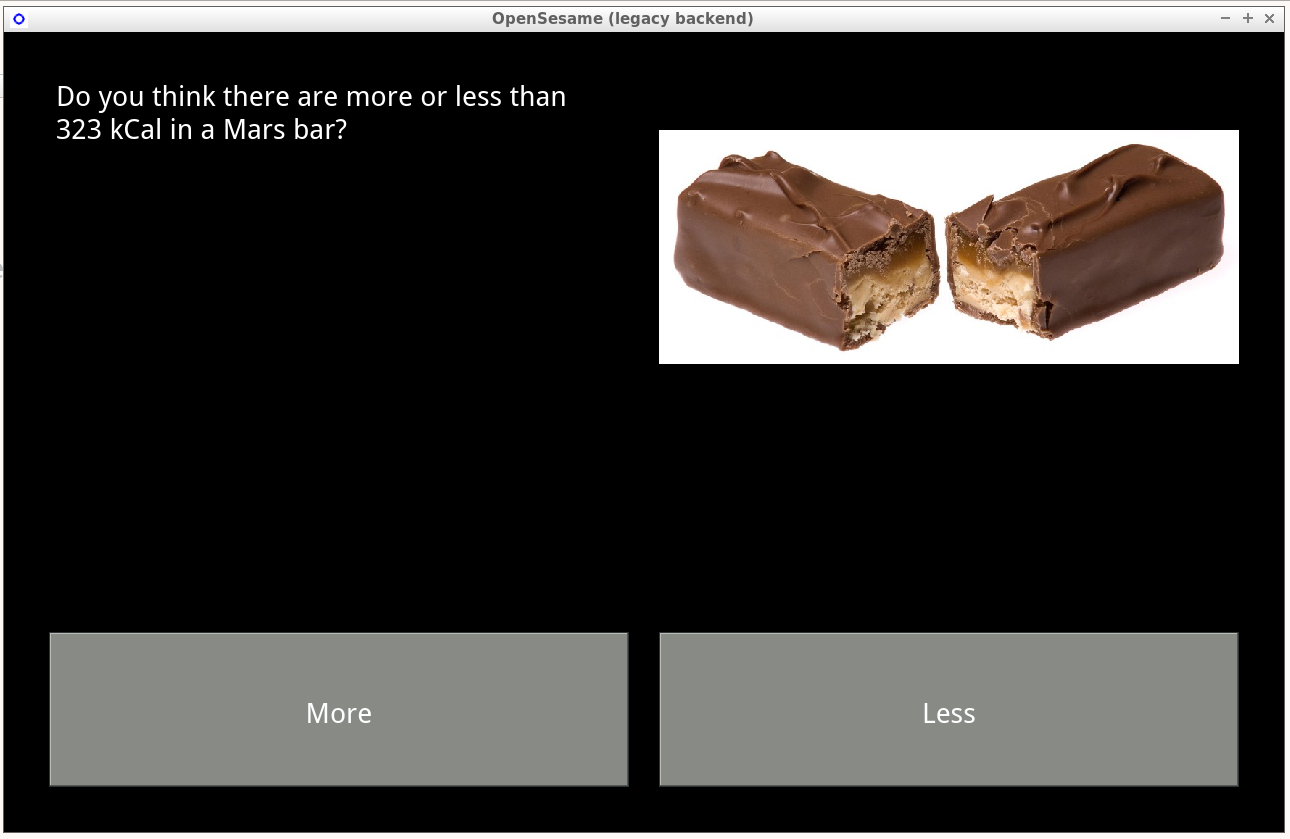
\includegraphics[width=0.95\linewidth]{Images/anchor_question.png}
 \end{subfigure}
 \begin{subfigure}[b]{0.49\textwidth}
 \caption{Calorie estimation}
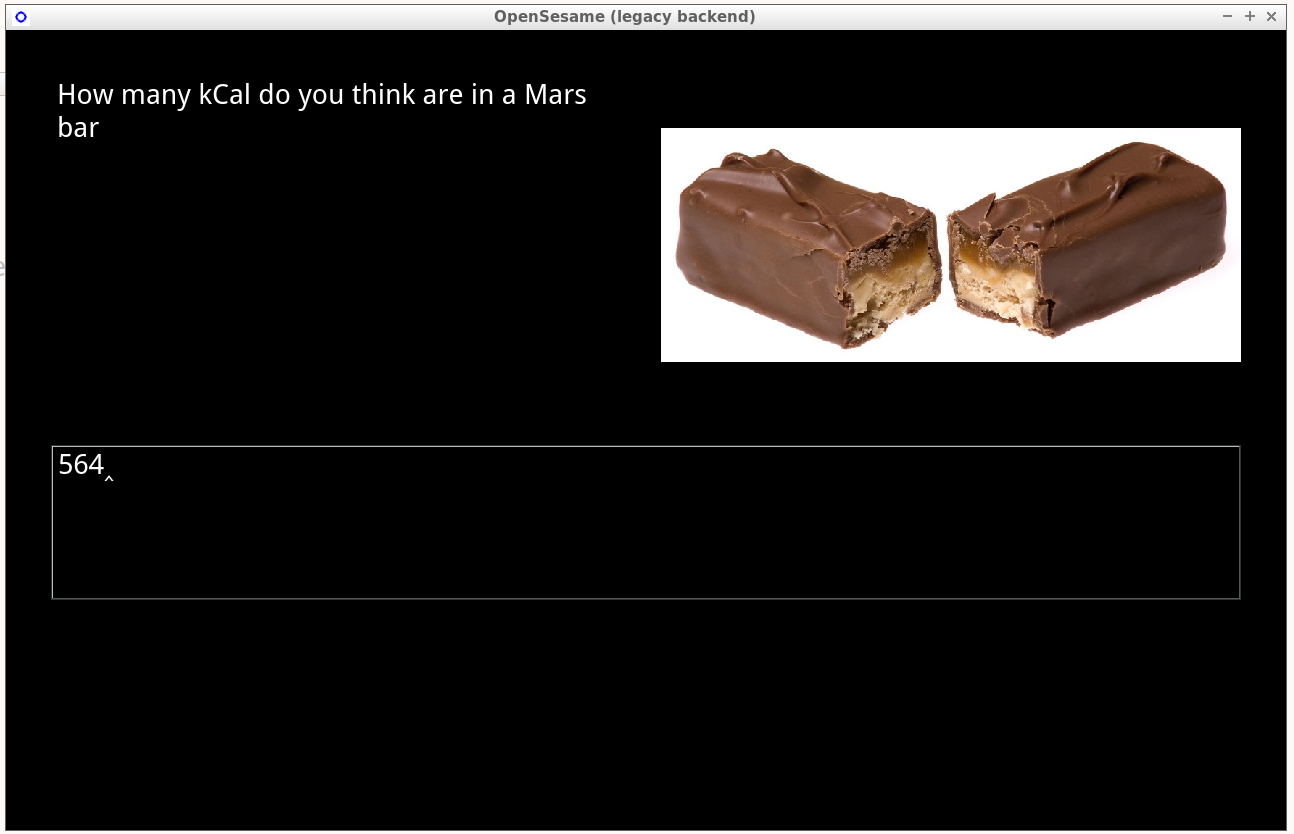
\includegraphics[width=0.95\linewidth]{Images/guess_question.png}
 \end{subfigure}
 \caption{Presentation of the questions on the screen.}
\label{fig:screenshots}
\end{figure}

\subsection{Design}

Upon starting the software, participants will be randomly assigned to one of three groups (not shown to the participants). The distribution of the various anchor conditions across the three groups is shown in Table~\ref{tab:design}. Each participant will be presented with each food once, and each type of anchor (high, low, no anchor) three times. For each participant, the order of in which the foods will be presented, will be randomised.

\begin{table}[!h]
  \caption{Distribution of anchors across the three groups. Participants will be randomly assigned to one of these groups when starting the software. `Neutral' means that no anchor question will be used.} 
  \label{tab:design} 
\begin{tabular}{p{5cm}p{3cm}p{3cm}p{3cm}}  
\hline 
Image & Group 1 & Group 2 & Group 3 \\ 
\hline
banana & High & Low & Neutral \\ 
cake & Low & Neutral & High \\ 
cheese & Low & Neutral & High \\ 
fries & Neutral & High & Low \\ 
honey & Neutral & High & Low \\ 
mars & High & Low & Neutral \\ 
peanuts & High & Low & Neutral \\ 
pizza & Neutral & High & Low \\ 
wine & Low & Neutral & High \\ 
\hline 
\end{tabular} 
\end{table} 

\subsection{Procedure}

Participants took part as part of a class on data visualisation methods. In order to get familiar with the data that would be used to demonstrate different data visualisation methods, they were asked to install the Opensesame software \citep{mathot12} on their laptop or to use the computers provided in the classroom. They then downloaded the program and loaded into Opensesame, after which they started the software.

After providing consent in the first screen of the program, they indicated of nine foods whether their calorie contents was lower or higher than a given value (for six of the foods shown to them) and then guess the calorie contents from the image of the food and the description of the food. 

After completing the calorie estimation of these foods, they answered a series of questions asking for their gender (male, female, do not wish to say), their age (could be left empty), whether they were currently or recently on a calorie restricting diet (also allowing no answer), how confident they were in their ability to estimate the calorie contents of foods, and which type of information they checked on food labels (calories, saturated fat, total fat, sugars, sodium).

They then sent the results file, which only contained a randomly chosen participant to the experimenter, who split the data between the guesses and the demographics information and removed the e-mail after processing the data. The combined document with guesses was made available to the public for teaching purposes, whereas the demographics were only shared within the group of participants who took part in the course.

\subsection{Data analysis}

The data will be processed using the R software (version 3.6.3). The focus will be on data visualisation, together with statistical comparisons (such as t-tests, ANOVAs) to examine whether observed differences are statistically significant. In particular, the following analyses will be used for each of the research questions.

\begin{description}
\item[RQ1. Does the anchoring effect occur for calorie estimation in foods?] Per food, estimates in the low and high anchor conditions will be plotted in the form of bar plots with error bars and independent samples t-tests will test the statistical significance of observed differences.
\item[RQ2. Does this anchoring effect depend on the type of food?] A scatterplot will reveal whether the anchoring effect depends on the actual calorie contents of the foods, while a significance test for correlations will be used to assess whether any relation is statistically significant. A descriptive approach will be taken to examine whether healthier foods have a smaller anchoring effect, since the use of nine foods does not allow for a systematic investigation.
\item[RQ3. Does high confidence lead to a smaller anchoring effect?] Participants will be split into groups based on how confidence they indicate to be. The groups will then be compared in bar graphs, grouped by confidence level, and statistically using t-tests or ANOVAs.
\item[RQ4. Do people who check food labels have a smaller anchoring effect?] Also here, participants will be split into groups, based on whether they report looking at calories on food labels. Groups will be compared with bar graphs and t-tests.
\end{description}

\section{Time schedule}

The study will run across two years, with data collected during the first week of each run of the course `interactive visualisation'. Data analysis will take place in subsequent years, after which a report will be produced (see Figure~\ref{fig:time_course}).

\begin{figure}[h!]
 \caption{Anchor question}
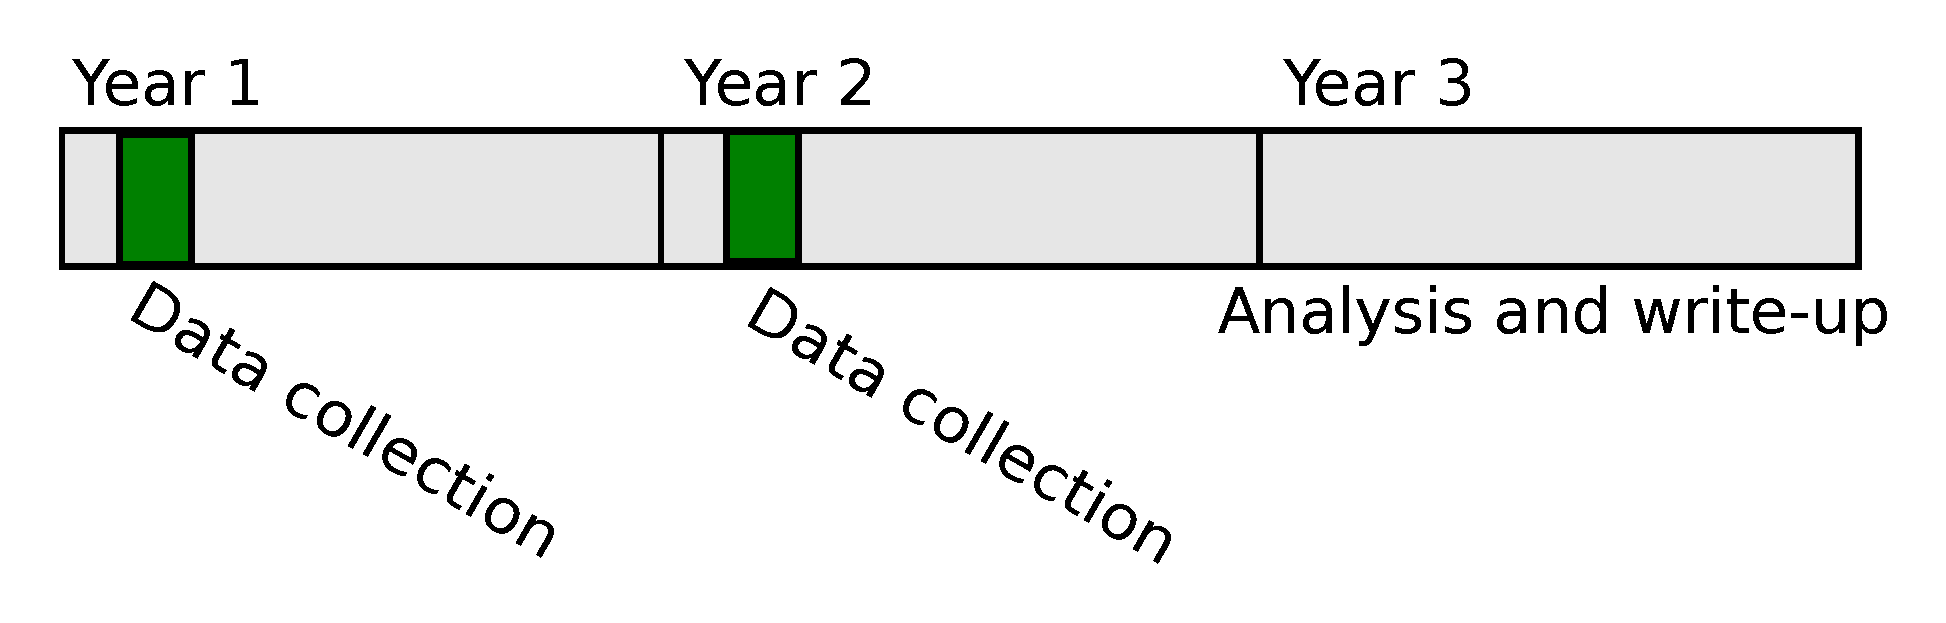
\includegraphics[width=0.95\linewidth]{Images/time_course.pdf}
 \caption{Proposed time-course of the project. Two data collection sessions are planned during the first week of the course. Time after these data collection sessions will be used for analysis and write-up. The project is expected to be completed in three years.}
\label{fig:time_course}
\end{figure}

\section{Risk analysis}

The main risk is that there will be insufficient participants in the study to reliably measure the anchoring effect for each type of food. Effect sizes in the past study \citep{shanks2020incidental} were low, and may possibly reflect an underestimation of the actual effect size. Not all participants of the course may be willing to take part or may be willing to share their data. In order to motivate people to take part, it will be explained that the data that they will produce will help them with the course. Two years of the course will be used to collect data from as many participants as possible.

A small number of foods will be tested. This has the advantage that participants may be more inclined to take part and complete the study. The disadvantage is that differences between foods (e.g., healthy versus less healthy) cannot be systematically investigated. For the anchoring effect, it is important that participants do not look up the actual calorie contents of the foods. The study must therefore be run in a lab setting rather than as an online survey. This is a restriction that cannot be overcome easily. A follow-up study could try and attract funding so that participants can be paid for participation, so that a longer session with more foods may become an option.

A further risk is that the software will not record the responses correctly. A related risk is that the software will not be able to deal with certain responses of the participants. To reduce this risk, the software will be tested extensively before starting data collection and the resulting data files inspected for any possible issues.

Another possible risk is that participants enter unrealistic estimates or enter texts rather than numbers as responses. The software does not provide an option to only allow numbers as entry. Data will therefore be inspected for incorrect entries. Outlier values will be identified using histograms and removed before mean values are computed. Accidental entry of letters will be corrected for.


\bibliography{anchoring}


\end{document}




